\subsection*{Task 1}

Too lazy to draw in tikz, so here you are.

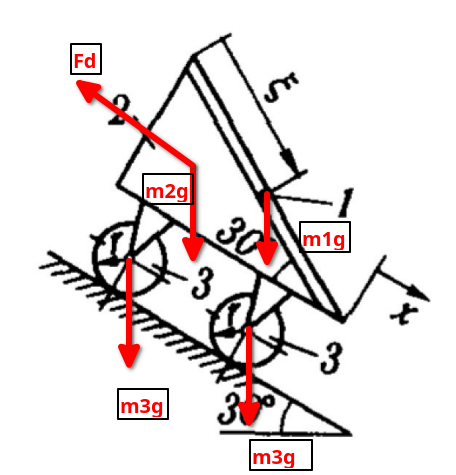
\includegraphics[width=\linewidth]{task1.png}

\subsubsection*{Part 1: find the angle to shoot the officer}

\begin{enumerate}
    \item RO: particle - planar motion
    \item Condition:
          \begin{center}
              \begin{tabular}{ |c|c|c| }
                  \hline
                  $$    & $initial$                & $final$                  \\
                  \hline
                  $t$   & $0$                      & $?$                      \\
                  \hline
                  $x$   & $0$                      & $L$                      \\
                  \hline
                  $x'$  & $v_0 \cdot \cos(\alpha)$ & $v_0 \cdot \cos(\alpha)$ \\
                  \hline
                  $x''$ & $0$                      & $0$                      \\
                  \hline
                  $y$   & $0$                      & $0$                      \\
                  \hline
                  $y'$  & $v_0 \cdot \sin(\alpha)$ & $?$                      \\
                  \hline
                  $y''$ & $-g$                     & $-g$                     \\
                  \hline
              \end{tabular}
          \end{center}
    \item Force analysis:
          $\vec{G}$
    \item Solution:
          \begin{enumerate}
              \item Equations by axis:
                    \begin{align}
                        \begin{cases}
                            mx'' = 0   \\
                            my'' = -mg \\
                        \end{cases}
                    \end{align}
                    Integration yields:
                    \begin{align}
                        \begin{cases}
                            x' = c_1       \\
                            y' = -gt + c_3 \\
                        \end{cases}
                    \end{align}
                    Another integration: \\
                    \begin{align}
                        \begin{cases}
                            x = c_1 t + c_2                    \\
                            y = -\frac{1}{2}gt^2 + c_3 t + c_4 \\
                        \end{cases}
                    \end{align}
              \item Substitution of initial values:
                    \begin{align}
                        \begin{cases}
                            c_1 = v_0 \cdot \cos(\alpha) \\
                            c_2 = 0                      \\
                            c_3 = v_0 \cdot \sin(\alpha) \\
                            c_4 = 0
                        \end{cases}
                    \end{align}
              \item Combining:
                    \begin{align}
                        \begin{cases}
                            L = v_0 \cdot \cos(\alpha) t \\
                            0 = -\frac{1}{2}gt^2 + v_0 \cdot \sin(\alpha) t
                        \end{cases}
                    \end{align}
              \item Result:
                    Python says there are two solutions: $\alpha = 0.0097$ and $\alpha = 1.561$.
                    And I have no doubts to not trust Python.
          \end{enumerate}
\end{enumerate}

\subsubsection*{Part 2: find the max height of the cargo ship can be to make this shot}

\begin{enumerate}
    \item As there are two angles that satisfy the first part, we need to find the max height for each of them.
    \item Analysis of equation for y-axis:
          \begin{align}
              y = -\frac{1}{2}gt^2 + v_0 \cdot \sin(\alpha) t
          \end{align}
    \item  As y is parabola, we can simply find its maximum height by finding extrema:
          \begin{align}
              t_{max} = \frac{v_0 \cdot \sin(\alpha)}{g} \\
              y_{max} = y(t_{max})
          \end{align}
    \item Result: \\
          For the first case: $y_{max} = 3.64555853045729$ \\
          For the second case: $y_{max} = 38574.3360928457$
\end{enumerate}

\subsubsection*{Part 3: find an angle $\alpha$, if you take into consideration the air resistance}

\begin{enumerate}
    \item RO: particle - planar motion
    \item Condition:
          \begin{center}
              \begin{tabular}{ |c|c|c| }
                  \hline
                  $$    & $initial$                & $final$ \\
                  \hline
                  $t$   & $0$                      & $?$     \\
                  \hline
                  $x$   & $0$                      & $L$     \\
                  \hline
                  $x'$  & $v_0 \cdot \cos(\alpha)$ & $?$     \\
                  \hline
                  $x''$ & $0$                      & $0$     \\
                  \hline
                  $y$   & $0$                      & $0$     \\
                  \hline
                  $y'$  & $v_0 \cdot \sin(\alpha)$ & $?$     \\
                  \hline
                  $y''$ & $-g$                     & $-g$    \\
                  \hline
              \end{tabular}
          \end{center}
    \item Force analysis:
          $\vec{G}$, $\vec{F}_{c}$
    \item Solution:
          \begin{enumerate}
              \item Equations by axis:
                    \begin{align}
                        \begin{cases}
                            mx'' = -k \sqrt{x'^2 + y'^2} x' \\
                            my'' = -mg - k \sqrt{x'^2 + y'^2} y'
                        \end{cases}
                    \end{align}
              \item Too hard to integrate by hands, so I'll use Python.
                    Everthing is the same as in part 1, but with different result.
              \item Result: \\
                    An angle to shoot officer is $\approx 0.0324$
          \end{enumerate}
    \item Air resistance force: \\
          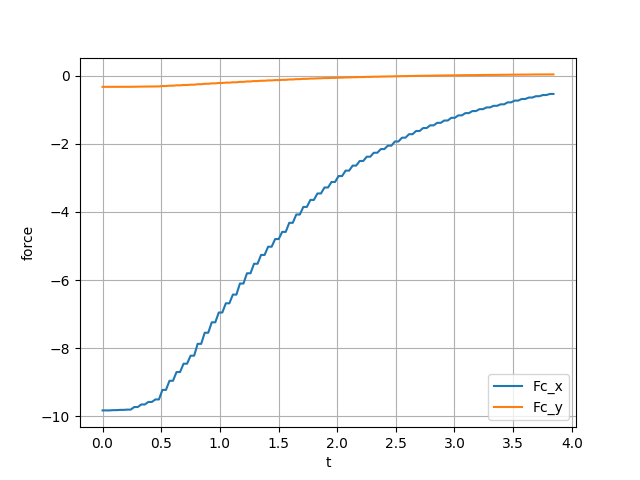
\includegraphics[width=\linewidth]{task1force.png}
    \item Trajectory with resistance: \\
          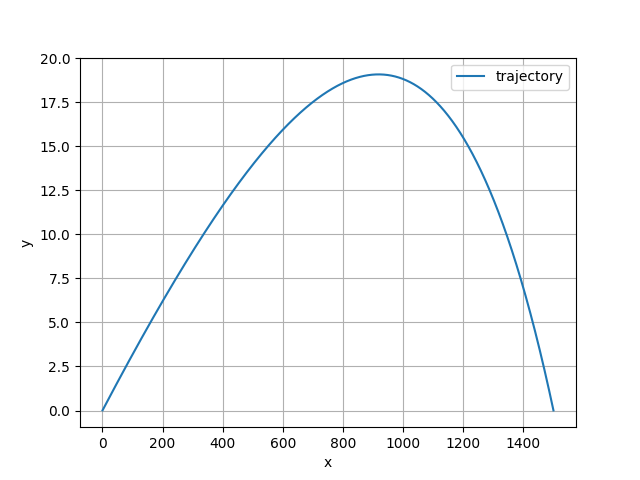
\includegraphics[width=\linewidth]{trajectory.png}
\end{enumerate}

\begin{answer}
    \begin{enumerate}
        \item
              $\alpha = 0.0097$, \\
              $\alpha = 1.561$
        \item
              $y_{max} = 38574.336$
        \item
              $\alpha = 0.0324$
    \end{enumerate}
\end{answer}